\documentclass[twoside]{book}

% Packages required by doxygen
\usepackage{fixltx2e}
\usepackage{calc}
\usepackage{doxygen}
\usepackage[export]{adjustbox} % also loads graphicx
\usepackage{graphicx}
\usepackage[utf8]{inputenc}
\usepackage{makeidx}
\usepackage{multicol}
\usepackage{multirow}
\PassOptionsToPackage{warn}{textcomp}
\usepackage{textcomp}
\usepackage[nointegrals]{wasysym}
\usepackage[table]{xcolor}

% Font selection
\usepackage[T1]{fontenc}
\usepackage[scaled=.90]{helvet}
\usepackage{courier}
\usepackage{amssymb}
\usepackage{sectsty}
\renewcommand{\familydefault}{\sfdefault}
\allsectionsfont{%
  \fontseries{bc}\selectfont%
  \color{darkgray}%
}
\renewcommand{\DoxyLabelFont}{%
  \fontseries{bc}\selectfont%
  \color{darkgray}%
}
\newcommand{\+}{\discretionary{\mbox{\scriptsize$\hookleftarrow$}}{}{}}

% Page & text layout
\usepackage{geometry}
\geometry{%
  a4paper,%
  top=2.5cm,%
  bottom=2.5cm,%
  left=2.5cm,%
  right=2.5cm%
}
\tolerance=750
\hfuzz=15pt
\hbadness=750
\setlength{\emergencystretch}{15pt}
\setlength{\parindent}{0cm}
\setlength{\parskip}{3ex plus 2ex minus 2ex}
\makeatletter
\renewcommand{\paragraph}{%
  \@startsection{paragraph}{4}{0ex}{-1.0ex}{1.0ex}{%
    \normalfont\normalsize\bfseries\SS@parafont%
  }%
}
\renewcommand{\subparagraph}{%
  \@startsection{subparagraph}{5}{0ex}{-1.0ex}{1.0ex}{%
    \normalfont\normalsize\bfseries\SS@subparafont%
  }%
}
\makeatother

% Headers & footers
\usepackage{fancyhdr}
\pagestyle{fancyplain}
\fancyhead[LE]{\fancyplain{}{\bfseries\thepage}}
\fancyhead[CE]{\fancyplain{}{}}
\fancyhead[RE]{\fancyplain{}{\bfseries\leftmark}}
\fancyhead[LO]{\fancyplain{}{\bfseries\rightmark}}
\fancyhead[CO]{\fancyplain{}{}}
\fancyhead[RO]{\fancyplain{}{\bfseries\thepage}}
\fancyfoot[LE]{\fancyplain{}{}}
\fancyfoot[CE]{\fancyplain{}{}}
\fancyfoot[RE]{\fancyplain{}{\bfseries\scriptsize Generated by Doxygen }}
\fancyfoot[LO]{\fancyplain{}{\bfseries\scriptsize Generated by Doxygen }}
\fancyfoot[CO]{\fancyplain{}{}}
\fancyfoot[RO]{\fancyplain{}{}}
\renewcommand{\footrulewidth}{0.4pt}
\renewcommand{\chaptermark}[1]{%
  \markboth{#1}{}%
}
\renewcommand{\sectionmark}[1]{%
  \markright{\thesection\ #1}%
}

% Indices & bibliography
\usepackage{natbib}
\usepackage[titles]{tocloft}
\setcounter{tocdepth}{3}
\setcounter{secnumdepth}{5}
\makeindex

% Hyperlinks (required, but should be loaded last)
\usepackage{ifpdf}
\ifpdf
  \usepackage[pdftex,pagebackref=true]{hyperref}
\else
  \usepackage[ps2pdf,pagebackref=true]{hyperref}
\fi
\hypersetup{%
  colorlinks=true,%
  linkcolor=blue,%
  citecolor=blue,%
  unicode%
}

% Custom commands
\newcommand{\clearemptydoublepage}{%
  \newpage{\pagestyle{empty}\cleardoublepage}%
}

\usepackage{caption}
\captionsetup{labelsep=space,justification=centering,font={bf},singlelinecheck=off,skip=4pt,position=top}

%===== C O N T E N T S =====

\begin{document}

% Titlepage & ToC
\hypersetup{pageanchor=false,
             bookmarksnumbered=true,
             pdfencoding=unicode
            }
\pagenumbering{roman}
\begin{titlepage}
\vspace*{7cm}
\begin{center}%
{\Large Armagetron\+Client }\\
\vspace*{1cm}
{\large Generated by Doxygen 1.8.11}\\
\end{center}
\end{titlepage}
\clearemptydoublepage
\tableofcontents
\clearemptydoublepage
\pagenumbering{arabic}
\hypersetup{pageanchor=true}

%--- Begin generated contents ---
\chapter{R\+E\+A\+D\+ME}
\label{md_D:_owncloud_HEIG-VD_JavaProjects_GEN_Armagetron_Client_README}
\hypertarget{md_D:_owncloud_HEIG-VD_JavaProjects_GEN_Armagetron_Client_README}{}
\input{md_D:_owncloud_HEIG-VD_JavaProjects_GEN_Armagetron_Client_README}
\chapter{Namespace Index}
\section{Packages}
Here are the packages with brief descriptions (if available)\+:\begin{DoxyCompactList}
\item\contentsline{section}{\hyperlink{namespaceclient}{client} }{\pageref{namespaceclient}}{}
\item\contentsline{section}{\hyperlink{namespacelogin}{login} }{\pageref{namespacelogin}}{}
\item\contentsline{section}{\hyperlink{namespacesample}{sample} }{\pageref{namespacesample}}{}
\end{DoxyCompactList}

\chapter{Hierarchical Index}
\section{Class Hierarchy}
This inheritance list is sorted roughly, but not completely, alphabetically\+:\begin{DoxyCompactList}
\item \contentsline{section}{sample.\+Controller}{\pageref{classsample_1_1_controller}}{}
\item \contentsline{section}{sample.\+Controller\+Test}{\pageref{classsample_1_1_controller_test}}{}
\item \contentsline{section}{client.\+Game}{\pageref{classclient_1_1_game}}{}
\item \contentsline{section}{client.\+Game\+Test}{\pageref{classclient_1_1_game_test}}{}
\item \contentsline{section}{login.\+Login\+Controller\+Test}{\pageref{classlogin_1_1_login_controller_test}}{}
\item Observable\begin{DoxyCompactList}
\item \contentsline{section}{login.\+Login\+Controller}{\pageref{classlogin_1_1_login_controller}}{}
\end{DoxyCompactList}
\item \contentsline{section}{client.\+Player}{\pageref{classclient_1_1_player}}{}
\item \contentsline{section}{client.\+Player\+Test}{\pageref{classclient_1_1_player_test}}{}
\item Runnable\begin{DoxyCompactList}
\item \contentsline{section}{client.\+Client}{\pageref{classclient_1_1_client}}{}
\end{DoxyCompactList}
\item Application\begin{DoxyCompactList}
\item \contentsline{section}{sample.\+Main}{\pageref{classsample_1_1_main}}{}
\end{DoxyCompactList}
\item Observer\begin{DoxyCompactList}
\item \contentsline{section}{sample.\+Main}{\pageref{classsample_1_1_main}}{}
\end{DoxyCompactList}
\end{DoxyCompactList}

\chapter{Class Index}
\section{Class List}
Here are the classes, structs, unions and interfaces with brief descriptions\+:\begin{DoxyCompactList}
\item\contentsline{section}{\hyperlink{classclient_1_1_client}{client.\+Client} }{\pageref{classclient_1_1_client}}{}
\item\contentsline{section}{\hyperlink{classsample_1_1_controller}{sample.\+Controller} }{\pageref{classsample_1_1_controller}}{}
\item\contentsline{section}{\hyperlink{classsample_1_1_controller_test}{sample.\+Controller\+Test} }{\pageref{classsample_1_1_controller_test}}{}
\item\contentsline{section}{\hyperlink{classclient_1_1_game}{client.\+Game} }{\pageref{classclient_1_1_game}}{}
\item\contentsline{section}{\hyperlink{classclient_1_1_game_test}{client.\+Game\+Test} }{\pageref{classclient_1_1_game_test}}{}
\item\contentsline{section}{\hyperlink{classlogin_1_1_login_controller}{login.\+Login\+Controller} }{\pageref{classlogin_1_1_login_controller}}{}
\item\contentsline{section}{\hyperlink{classlogin_1_1_login_controller_test}{login.\+Login\+Controller\+Test} }{\pageref{classlogin_1_1_login_controller_test}}{}
\item\contentsline{section}{\hyperlink{classsample_1_1_main}{sample.\+Main} }{\pageref{classsample_1_1_main}}{}
\item\contentsline{section}{\hyperlink{classclient_1_1_player}{client.\+Player} }{\pageref{classclient_1_1_player}}{}
\item\contentsline{section}{\hyperlink{classclient_1_1_player_test}{client.\+Player\+Test} }{\pageref{classclient_1_1_player_test}}{}
\end{DoxyCompactList}

\chapter{File Index}
\section{File List}
Here is a list of all files with brief descriptions\+:\begin{DoxyCompactList}
\item\contentsline{section}{D\+:/owncloud/\+H\+E\+I\+G-\/\+V\+D/\+Java\+Projects/\+G\+E\+N\+\_\+\+Armagetron\+\_\+\+Client/src/main/java/client/\hyperlink{_client_8java}{Client.\+java} \\*\+: Client Class that generate the play ground window }{\pageref{_client_8java}}{}
\item\contentsline{section}{D\+:/owncloud/\+H\+E\+I\+G-\/\+V\+D/\+Java\+Projects/\+G\+E\+N\+\_\+\+Armagetron\+\_\+\+Client/src/main/java/client/\hyperlink{_game_8java}{Game.\+java} \\*\+: Game class that manage local data for players }{\pageref{_game_8java}}{}
\item\contentsline{section}{D\+:/owncloud/\+H\+E\+I\+G-\/\+V\+D/\+Java\+Projects/\+G\+E\+N\+\_\+\+Armagetron\+\_\+\+Client/src/main/java/client/\hyperlink{_player_8java}{Player.\+java} \\*\+: Player class }{\pageref{_player_8java}}{}
\item\contentsline{section}{D\+:/owncloud/\+H\+E\+I\+G-\/\+V\+D/\+Java\+Projects/\+G\+E\+N\+\_\+\+Armagetron\+\_\+\+Client/src/main/java/login/\hyperlink{_login_controller_8java}{Login\+Controller.\+java} \\*\+: Controller of the login windows }{\pageref{_login_controller_8java}}{}
\item\contentsline{section}{D\+:/owncloud/\+H\+E\+I\+G-\/\+V\+D/\+Java\+Projects/\+G\+E\+N\+\_\+\+Armagetron\+\_\+\+Client/src/main/java/sample/\hyperlink{_controller_8java}{Controller.\+java} \\*\+: Controller of the playing grid that display the game }{\pageref{_controller_8java}}{}
\item\contentsline{section}{D\+:/owncloud/\+H\+E\+I\+G-\/\+V\+D/\+Java\+Projects/\+G\+E\+N\+\_\+\+Armagetron\+\_\+\+Client/src/main/java/sample/\hyperlink{_main_8java}{Main.\+java} \\*\+: M\+A\+IN class that run the client }{\pageref{_main_8java}}{}
\item\contentsline{section}{D\+:/owncloud/\+H\+E\+I\+G-\/\+V\+D/\+Java\+Projects/\+G\+E\+N\+\_\+\+Armagetron\+\_\+\+Client/src/test/java/client/\hyperlink{_game_test_8java}{Game\+Test.\+java} }{\pageref{_game_test_8java}}{}
\item\contentsline{section}{D\+:/owncloud/\+H\+E\+I\+G-\/\+V\+D/\+Java\+Projects/\+G\+E\+N\+\_\+\+Armagetron\+\_\+\+Client/src/test/java/client/\hyperlink{_player_test_8java}{Player\+Test.\+java} }{\pageref{_player_test_8java}}{}
\item\contentsline{section}{D\+:/owncloud/\+H\+E\+I\+G-\/\+V\+D/\+Java\+Projects/\+G\+E\+N\+\_\+\+Armagetron\+\_\+\+Client/src/test/java/login/\hyperlink{_login_controller_test_8java}{Login\+Controller\+Test.\+java} }{\pageref{_login_controller_test_8java}}{}
\item\contentsline{section}{D\+:/owncloud/\+H\+E\+I\+G-\/\+V\+D/\+Java\+Projects/\+G\+E\+N\+\_\+\+Armagetron\+\_\+\+Client/src/test/java/sample/\hyperlink{_controller_test_8java}{Controller\+Test.\+java} }{\pageref{_controller_test_8java}}{}
\end{DoxyCompactList}

\chapter{Namespace Documentation}
\hypertarget{namespaceclient}{}\section{Package client}
\label{namespaceclient}\index{client@{client}}
\subsection*{Classes}
\begin{DoxyCompactItemize}
\item 
class \hyperlink{classclient_1_1_client}{Client}
\item 
class \hyperlink{classclient_1_1_game}{Game}
\item 
class \hyperlink{classclient_1_1_game_test}{Game\+Test}
\item 
class \hyperlink{classclient_1_1_player}{Player}
\item 
class \hyperlink{classclient_1_1_player_test}{Player\+Test}
\end{DoxyCompactItemize}

\hypertarget{namespacelogin}{}\section{Package login}
\label{namespacelogin}\index{login@{login}}
\subsection*{Classes}
\begin{DoxyCompactItemize}
\item 
class \hyperlink{classlogin_1_1_login_controller}{Login\+Controller}
\item 
class \hyperlink{classlogin_1_1_login_controller_test}{Login\+Controller\+Test}
\end{DoxyCompactItemize}

\hypertarget{namespacesample}{}\section{Package sample}
\label{namespacesample}\index{sample@{sample}}
\subsection*{Classes}
\begin{DoxyCompactItemize}
\item 
class \hyperlink{classsample_1_1_controller}{Controller}
\item 
class \hyperlink{classsample_1_1_controller_test}{Controller\+Test}
\item 
class \hyperlink{classsample_1_1_main}{Main}
\end{DoxyCompactItemize}

\chapter{Class Documentation}
\hypertarget{classclient_1_1_client}{}\section{client.\+Client Class Reference}
\label{classclient_1_1_client}\index{client.\+Client@{client.\+Client}}
Inheritance diagram for client.\+Client\+:\begin{figure}[H]
\begin{center}
\leavevmode
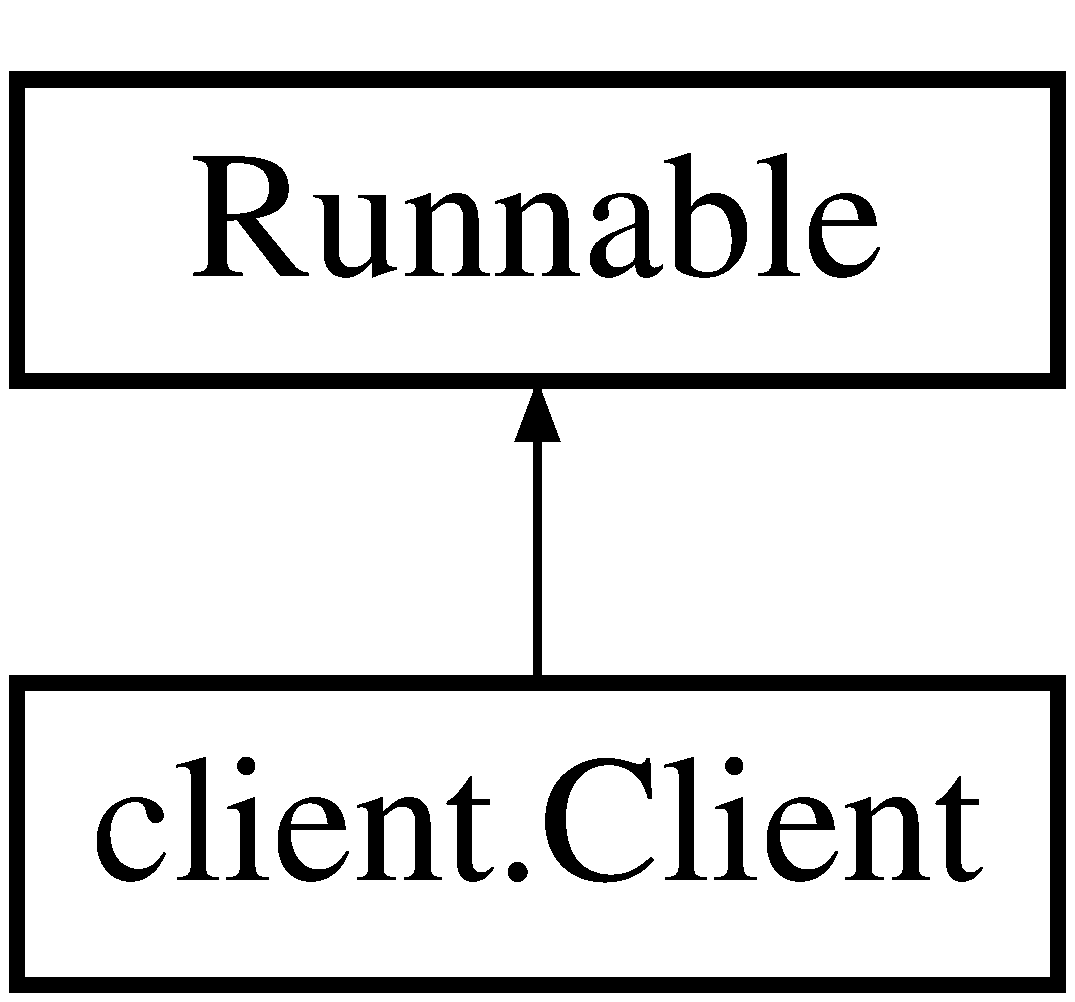
\includegraphics[height=2.000000cm]{classclient_1_1_client}
\end{center}
\end{figure}
\subsection*{Public Member Functions}
\begin{DoxyCompactItemize}
\item 
\hyperlink{classclient_1_1_client_a85d8183914ca2a3444baf7599ff3d142}{Client} (String server\+Address, int port, String username, \hyperlink{classsample_1_1_controller}{Controller} controller, Color user\+Color)
\item 
void \hyperlink{classclient_1_1_client_a81b53ebbce32b100fbdb3835c57583d9}{send\+Data} (Object o)
\begin{DoxyCompactList}\small\item\em Send Data to the server. \end{DoxyCompactList}\item 
void \hyperlink{classclient_1_1_client_af1d54c5ce231e58cacd819675c3f98ab}{run} ()
\end{DoxyCompactItemize}


\subsection{Detailed Description}


Definition at line 22 of file Client.\+java.



\subsection{Constructor \& Destructor Documentation}
\index{client\+::\+Client@{client\+::\+Client}!Client@{Client}}
\index{Client@{Client}!client\+::\+Client@{client\+::\+Client}}
\subsubsection[{\texorpdfstring{Client(\+String server\+Address, int port, String username, Controller controller, Color user\+Color)}{Client(String serverAddress, int port, String username, Controller controller, Color userColor)}}]{\setlength{\rightskip}{0pt plus 5cm}client.\+Client.\+Client (
\begin{DoxyParamCaption}
\item[{String}]{server\+Address, }
\item[{int}]{port, }
\item[{String}]{username, }
\item[{{\bf Controller}}]{controller, }
\item[{Color}]{user\+Color}
\end{DoxyParamCaption}
)}\hypertarget{classclient_1_1_client_a85d8183914ca2a3444baf7599ff3d142}{}\label{classclient_1_1_client_a85d8183914ca2a3444baf7599ff3d142}


Definition at line 38 of file Client.\+java.



\subsection{Member Function Documentation}
\index{client\+::\+Client@{client\+::\+Client}!run@{run}}
\index{run@{run}!client\+::\+Client@{client\+::\+Client}}
\subsubsection[{\texorpdfstring{run()}{run()}}]{\setlength{\rightskip}{0pt plus 5cm}void client.\+Client.\+run (
\begin{DoxyParamCaption}
{}
\end{DoxyParamCaption}
)}\hypertarget{classclient_1_1_client_af1d54c5ce231e58cacd819675c3f98ab}{}\label{classclient_1_1_client_af1d54c5ce231e58cacd819675c3f98ab}


Definition at line 133 of file Client.\+java.

\index{client\+::\+Client@{client\+::\+Client}!send\+Data@{send\+Data}}
\index{send\+Data@{send\+Data}!client\+::\+Client@{client\+::\+Client}}
\subsubsection[{\texorpdfstring{send\+Data(\+Object o)}{sendData(Object o)}}]{\setlength{\rightskip}{0pt plus 5cm}void client.\+Client.\+send\+Data (
\begin{DoxyParamCaption}
\item[{Object}]{o}
\end{DoxyParamCaption}
)}\hypertarget{classclient_1_1_client_a81b53ebbce32b100fbdb3835c57583d9}{}\label{classclient_1_1_client_a81b53ebbce32b100fbdb3835c57583d9}


Send Data to the server. 


\begin{DoxyParams}{Parameters}
{\em o} & The object to send \\
\hline
\end{DoxyParams}


Definition at line 84 of file Client.\+java.



The documentation for this class was generated from the following file\+:\begin{DoxyCompactItemize}
\item 
D\+:/owncloud/\+H\+E\+I\+G-\/\+V\+D/\+Java\+Projects/\+G\+E\+N\+\_\+\+Armagetron\+\_\+\+Client/src/main/java/client/\hyperlink{_client_8java}{Client.\+java}\end{DoxyCompactItemize}

\hypertarget{classsample_1_1_controller}{}\section{sample.\+Controller Class Reference}
\label{classsample_1_1_controller}\index{sample.\+Controller@{sample.\+Controller}}
\subsection*{Public Member Functions}
\begin{DoxyCompactItemize}
\item 
void \hyperlink{classsample_1_1_controller_a65dad2fa17f9b15a2960c821fe35c7c9}{connect} (String server\+IP, String user\+Name, Color user\+Color)
\begin{DoxyCompactList}\small\item\em Connection between client and server. \end{DoxyCompactList}\item 
void \hyperlink{classsample_1_1_controller_a31ef16ada5fa90e7216d0c9b4e78fbd2}{on\+Key\+Pressed} (Key\+Event key\+Event)
\begin{DoxyCompactList}\small\item\em send to key pressed to the client object \end{DoxyCompactList}\item 
void \hyperlink{classsample_1_1_controller_a4e96857dfe66c3e7fcb60deaeca5d5c9}{process\+Data} (Object o)
\begin{DoxyCompactList}\small\item\em receive the objects from the client \end{DoxyCompactList}\item 
\hyperlink{classclient_1_1_client}{Client} \hyperlink{classsample_1_1_controller_adcbbb3b9c5b3a037b3c61560ba0f5c62}{get\+Client} ()
\begin{DoxyCompactList}\small\item\em Return the client. \end{DoxyCompactList}\end{DoxyCompactItemize}


\subsection{Detailed Description}


Definition at line 34 of file Controller.\+java.



\subsection{Member Function Documentation}
\index{sample\+::\+Controller@{sample\+::\+Controller}!connect@{connect}}
\index{connect@{connect}!sample\+::\+Controller@{sample\+::\+Controller}}
\subsubsection[{\texorpdfstring{connect(\+String server\+I\+P, String user\+Name, Color user\+Color)}{connect(String serverIP, String userName, Color userColor)}}]{\setlength{\rightskip}{0pt plus 5cm}sample.\+Controller.\+connect (
\begin{DoxyParamCaption}
\item[{String}]{server\+IP, }
\item[{String}]{user\+Name, }
\item[{Color}]{user\+Color}
\end{DoxyParamCaption}
)}\hypertarget{classsample_1_1_controller_a65dad2fa17f9b15a2960c821fe35c7c9}{}\label{classsample_1_1_controller_a65dad2fa17f9b15a2960c821fe35c7c9}


Connection between client and server. 


\begin{DoxyParams}{Parameters}
{\em server\+IP} & \\
\hline
{\em user\+Name} & \\
\hline
{\em user\+Color} & \\
\hline
\end{DoxyParams}


Definition at line 103 of file Controller.\+java.

\index{sample\+::\+Controller@{sample\+::\+Controller}!get\+Client@{get\+Client}}
\index{get\+Client@{get\+Client}!sample\+::\+Controller@{sample\+::\+Controller}}
\subsubsection[{\texorpdfstring{get\+Client()}{getClient()}}]{\setlength{\rightskip}{0pt plus 5cm}sample.\+Controller.\+get\+Client (
\begin{DoxyParamCaption}
{}
\end{DoxyParamCaption}
)}\hypertarget{classsample_1_1_controller_adcbbb3b9c5b3a037b3c61560ba0f5c62}{}\label{classsample_1_1_controller_adcbbb3b9c5b3a037b3c61560ba0f5c62}


Return the client. 



Definition at line 320 of file Controller.\+java.

\index{sample\+::\+Controller@{sample\+::\+Controller}!on\+Key\+Pressed@{on\+Key\+Pressed}}
\index{on\+Key\+Pressed@{on\+Key\+Pressed}!sample\+::\+Controller@{sample\+::\+Controller}}
\subsubsection[{\texorpdfstring{on\+Key\+Pressed(\+Key\+Event key\+Event)}{onKeyPressed(KeyEvent keyEvent)}}]{\setlength{\rightskip}{0pt plus 5cm}sample.\+Controller.\+on\+Key\+Pressed (
\begin{DoxyParamCaption}
\item[{Key\+Event}]{key\+Event}
\end{DoxyParamCaption}
)}\hypertarget{classsample_1_1_controller_a31ef16ada5fa90e7216d0c9b4e78fbd2}{}\label{classsample_1_1_controller_a31ef16ada5fa90e7216d0c9b4e78fbd2}


send to key pressed to the client object 


\begin{DoxyParams}{Parameters}
{\em key\+Event} & \\
\hline
\end{DoxyParams}


Definition at line 114 of file Controller.\+java.

\index{sample\+::\+Controller@{sample\+::\+Controller}!process\+Data@{process\+Data}}
\index{process\+Data@{process\+Data}!sample\+::\+Controller@{sample\+::\+Controller}}
\subsubsection[{\texorpdfstring{process\+Data(\+Object o)}{processData(Object o)}}]{\setlength{\rightskip}{0pt plus 5cm}sample.\+Controller.\+process\+Data (
\begin{DoxyParamCaption}
\item[{Object}]{o}
\end{DoxyParamCaption}
)}\hypertarget{classsample_1_1_controller_a4e96857dfe66c3e7fcb60deaeca5d5c9}{}\label{classsample_1_1_controller_a4e96857dfe66c3e7fcb60deaeca5d5c9}


receive the objects from the client 


\begin{DoxyParams}{Parameters}
{\em o} & \\
\hline
\end{DoxyParams}


Definition at line 157 of file Controller.\+java.



The documentation for this class was generated from the following file\+:\begin{DoxyCompactItemize}
\item 
D\+:/owncloud/\+H\+E\+I\+G-\/\+V\+D/\+Java\+Projects/\+G\+E\+N\+\_\+\+Armagetron\+\_\+\+Client/src/main/java/sample/\hyperlink{_controller_8java}{Controller.\+java}\end{DoxyCompactItemize}

\hypertarget{classsample_1_1_controller_test}{}\section{sample.\+Controller\+Test Class Reference}
\label{classsample_1_1_controller_test}\index{sample.\+Controller\+Test@{sample.\+Controller\+Test}}
\subsection*{Public Member Functions}
\begin{DoxyCompactItemize}
\item 
void \hyperlink{classsample_1_1_controller_test_a94c68449cab78c412846d29cd1b294b8}{init} ()  throws Exception 
\item 
void \hyperlink{classsample_1_1_controller_test_a3a2b1555d6b4bd15ccb7ff335d1eba6f}{connect} ()  throws Exception 
\end{DoxyCompactItemize}


\subsection{Detailed Description}


Definition at line 17 of file Controller\+Test.\+java.



\subsection{Member Function Documentation}
\index{sample\+::\+Controller\+Test@{sample\+::\+Controller\+Test}!connect@{connect}}
\index{connect@{connect}!sample\+::\+Controller\+Test@{sample\+::\+Controller\+Test}}
\subsubsection[{\texorpdfstring{connect()}{connect()}}]{\setlength{\rightskip}{0pt plus 5cm}void sample.\+Controller\+Test.\+connect (
\begin{DoxyParamCaption}
{}
\end{DoxyParamCaption}
) throws Exception}\hypertarget{classsample_1_1_controller_test_a3a2b1555d6b4bd15ccb7ff335d1eba6f}{}\label{classsample_1_1_controller_test_a3a2b1555d6b4bd15ccb7ff335d1eba6f}


Definition at line 26 of file Controller\+Test.\+java.

\index{sample\+::\+Controller\+Test@{sample\+::\+Controller\+Test}!init@{init}}
\index{init@{init}!sample\+::\+Controller\+Test@{sample\+::\+Controller\+Test}}
\subsubsection[{\texorpdfstring{init()}{init()}}]{\setlength{\rightskip}{0pt plus 5cm}void sample.\+Controller\+Test.\+init (
\begin{DoxyParamCaption}
{}
\end{DoxyParamCaption}
) throws Exception}\hypertarget{classsample_1_1_controller_test_a94c68449cab78c412846d29cd1b294b8}{}\label{classsample_1_1_controller_test_a94c68449cab78c412846d29cd1b294b8}


Definition at line 21 of file Controller\+Test.\+java.



The documentation for this class was generated from the following file\+:\begin{DoxyCompactItemize}
\item 
D\+:/owncloud/\+H\+E\+I\+G-\/\+V\+D/\+Java\+Projects/\+G\+E\+N\+\_\+\+Armagetron\+\_\+\+Client/src/test/java/sample/\hyperlink{_controller_test_8java}{Controller\+Test.\+java}\end{DoxyCompactItemize}

\hypertarget{classclient_1_1_game}{}\section{client.\+Game Class Reference}
\label{classclient_1_1_game}\index{client.\+Game@{client.\+Game}}
\subsection*{Public Member Functions}
\begin{DoxyCompactItemize}
\item 
\hyperlink{classclient_1_1_game_a59f4e247962a84ae39f37ef63b02d1a2}{Game} ()
\item 
Array\+List$<$ \hyperlink{classclient_1_1_player}{Player} $>$ \hyperlink{classclient_1_1_game_a0b740cbaa55e14618450b2dfd173795c}{get\+Players} ()
\begin{DoxyCompactList}\small\item\em Return a list of all players. \end{DoxyCompactList}\item 
void \hyperlink{classclient_1_1_game_a29980336f978894cb9c6196cbd4ff65e}{set\+Players} (Array\+List$<$ Player\+Data $>$ players\+Data)
\begin{DoxyCompactList}\small\item\em Create the players list from the players\+Data send from the server. \end{DoxyCompactList}\end{DoxyCompactItemize}


\subsection{Detailed Description}


Definition at line 16 of file Game.\+java.



\subsection{Constructor \& Destructor Documentation}
\index{client\+::\+Game@{client\+::\+Game}!Game@{Game}}
\index{Game@{Game}!client\+::\+Game@{client\+::\+Game}}
\subsubsection[{\texorpdfstring{Game()}{Game()}}]{\setlength{\rightskip}{0pt plus 5cm}client.\+Game.\+Game (
\begin{DoxyParamCaption}
{}
\end{DoxyParamCaption}
)}\hypertarget{classclient_1_1_game_a59f4e247962a84ae39f37ef63b02d1a2}{}\label{classclient_1_1_game_a59f4e247962a84ae39f37ef63b02d1a2}


Definition at line 19 of file Game.\+java.



\subsection{Member Function Documentation}
\index{client\+::\+Game@{client\+::\+Game}!get\+Players@{get\+Players}}
\index{get\+Players@{get\+Players}!client\+::\+Game@{client\+::\+Game}}
\subsubsection[{\texorpdfstring{get\+Players()}{getPlayers()}}]{\setlength{\rightskip}{0pt plus 5cm}public Array\+List$<$ {\bf Player} $>$ client.\+Game.\+get\+Players (
\begin{DoxyParamCaption}
{}
\end{DoxyParamCaption}
)}\hypertarget{classclient_1_1_game_a0b740cbaa55e14618450b2dfd173795c}{}\label{classclient_1_1_game_a0b740cbaa55e14618450b2dfd173795c}


Return a list of all players. 

\begin{DoxyReturn}{Returns}
Array\+List$<$\+Player$>$ The list of players 
\end{DoxyReturn}


Definition at line 30 of file Game.\+java.

\index{client\+::\+Game@{client\+::\+Game}!set\+Players@{set\+Players}}
\index{set\+Players@{set\+Players}!client\+::\+Game@{client\+::\+Game}}
\subsubsection[{\texorpdfstring{set\+Players(\+Array\+List$<$ Player\+Data $>$ players\+Data)}{setPlayers(ArrayList< PlayerData > playersData)}}]{\setlength{\rightskip}{0pt plus 5cm}client.\+Game.\+set\+Players (
\begin{DoxyParamCaption}
\item[{Array\+List$<$ Player\+Data $>$}]{players\+Data}
\end{DoxyParamCaption}
)}\hypertarget{classclient_1_1_game_a29980336f978894cb9c6196cbd4ff65e}{}\label{classclient_1_1_game_a29980336f978894cb9c6196cbd4ff65e}


Create the players list from the players\+Data send from the server. 


\begin{DoxyParams}{Parameters}
{\em players\+Data} & \\
\hline
\end{DoxyParams}


Definition at line 52 of file Game.\+java.



The documentation for this class was generated from the following file\+:\begin{DoxyCompactItemize}
\item 
D\+:/owncloud/\+H\+E\+I\+G-\/\+V\+D/\+Java\+Projects/\+G\+E\+N\+\_\+\+Armagetron\+\_\+\+Client/src/main/java/client/\hyperlink{_game_8java}{Game.\+java}\end{DoxyCompactItemize}

\hypertarget{classclient_1_1_game_test}{}\section{client.\+Game\+Test Class Reference}
\label{classclient_1_1_game_test}\index{client.\+Game\+Test@{client.\+Game\+Test}}
\subsection*{Public Member Functions}
\begin{DoxyCompactItemize}
\item 
void \hyperlink{classclient_1_1_game_test_a694a5c5f6f92a32602f52eb77a714445}{get\+Players} ()  throws Exception 
\end{DoxyCompactItemize}


\subsection{Detailed Description}


Definition at line 20 of file Game\+Test.\+java.



\subsection{Member Function Documentation}
\index{client\+::\+Game\+Test@{client\+::\+Game\+Test}!get\+Players@{get\+Players}}
\index{get\+Players@{get\+Players}!client\+::\+Game\+Test@{client\+::\+Game\+Test}}
\subsubsection[{\texorpdfstring{get\+Players()}{getPlayers()}}]{\setlength{\rightskip}{0pt plus 5cm}void client.\+Game\+Test.\+get\+Players (
\begin{DoxyParamCaption}
{}
\end{DoxyParamCaption}
) throws Exception}\hypertarget{classclient_1_1_game_test_a694a5c5f6f92a32602f52eb77a714445}{}\label{classclient_1_1_game_test_a694a5c5f6f92a32602f52eb77a714445}


Definition at line 29 of file Game\+Test.\+java.



The documentation for this class was generated from the following file\+:\begin{DoxyCompactItemize}
\item 
D\+:/owncloud/\+H\+E\+I\+G-\/\+V\+D/\+Java\+Projects/\+G\+E\+N\+\_\+\+Armagetron\+\_\+\+Client/src/test/java/client/\hyperlink{_game_test_8java}{Game\+Test.\+java}\end{DoxyCompactItemize}

\hypertarget{classlogin_1_1_login_controller}{}\section{login.\+Login\+Controller Class Reference}
\label{classlogin_1_1_login_controller}\index{login.\+Login\+Controller@{login.\+Login\+Controller}}
Inheritance diagram for login.\+Login\+Controller\+:\begin{figure}[H]
\begin{center}
\leavevmode
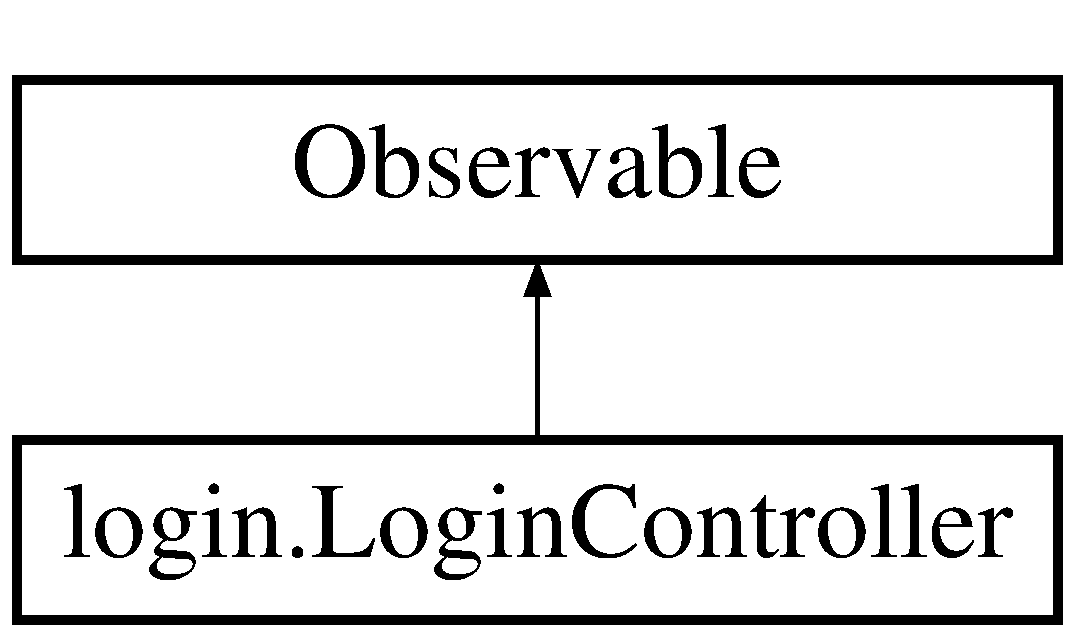
\includegraphics[height=2.000000cm]{classlogin_1_1_login_controller}
\end{center}
\end{figure}
\subsection*{Public Member Functions}
\begin{DoxyCompactItemize}
\item 
void \hyperlink{classlogin_1_1_login_controller_aad48ea189ef89f216cd9baa8a045a792}{init} ()
\begin{DoxyCompactList}\small\item\em Method that initate the \hyperlink{classlogin_1_1_login_controller}{Login\+Controller}. \end{DoxyCompactList}\item 
boolean \hyperlink{classlogin_1_1_login_controller_ace34b5fc7aaed7dad451c7bd4f18360b}{check\+Form} ()
\begin{DoxyCompactList}\small\item\em Methode to check if the state\textquotesingle{}s form. \end{DoxyCompactList}\end{DoxyCompactItemize}
\subsection*{Public Attributes}
\begin{DoxyCompactItemize}
\item 
String \hyperlink{classlogin_1_1_login_controller_aca2945118c790e029183a46347154ee3}{user\+Name}
\item 
String \hyperlink{classlogin_1_1_login_controller_abe699936676f2262b822fe0dcafd35b1}{server\+IP}
\item 
Color \hyperlink{classlogin_1_1_login_controller_a081ea0de3603e343739a9c123b52e622}{user\+Color}
\end{DoxyCompactItemize}


\subsection{Detailed Description}


Definition at line 25 of file Login\+Controller.\+java.



\subsection{Member Function Documentation}
\index{login\+::\+Login\+Controller@{login\+::\+Login\+Controller}!check\+Form@{check\+Form}}
\index{check\+Form@{check\+Form}!login\+::\+Login\+Controller@{login\+::\+Login\+Controller}}
\subsubsection[{\texorpdfstring{check\+Form()}{checkForm()}}]{\setlength{\rightskip}{0pt plus 5cm}public boolean login.\+Login\+Controller.\+check\+Form (
\begin{DoxyParamCaption}
{}
\end{DoxyParamCaption}
)}\hypertarget{classlogin_1_1_login_controller_ace34b5fc7aaed7dad451c7bd4f18360b}{}\label{classlogin_1_1_login_controller_ace34b5fc7aaed7dad451c7bd4f18360b}


Methode to check if the state\textquotesingle{}s form. 

\begin{DoxyReturn}{Returns}
boolean 
\end{DoxyReturn}


Definition at line 137 of file Login\+Controller.\+java.

\index{login\+::\+Login\+Controller@{login\+::\+Login\+Controller}!init@{init}}
\index{init@{init}!login\+::\+Login\+Controller@{login\+::\+Login\+Controller}}
\subsubsection[{\texorpdfstring{init()}{init()}}]{\setlength{\rightskip}{0pt plus 5cm}public void login.\+Login\+Controller.\+init (
\begin{DoxyParamCaption}
{}
\end{DoxyParamCaption}
)}\hypertarget{classlogin_1_1_login_controller_aad48ea189ef89f216cd9baa8a045a792}{}\label{classlogin_1_1_login_controller_aad48ea189ef89f216cd9baa8a045a792}


Method that initate the \hyperlink{classlogin_1_1_login_controller}{Login\+Controller}. 

\begin{DoxyReturn}{Returns}
void 
\end{DoxyReturn}


Definition at line 51 of file Login\+Controller.\+java.



\subsection{Member Data Documentation}
\index{login\+::\+Login\+Controller@{login\+::\+Login\+Controller}!server\+IP@{server\+IP}}
\index{server\+IP@{server\+IP}!login\+::\+Login\+Controller@{login\+::\+Login\+Controller}}
\subsubsection[{\texorpdfstring{server\+IP}{serverIP}}]{\setlength{\rightskip}{0pt plus 5cm}String login.\+Login\+Controller.\+server\+IP}\hypertarget{classlogin_1_1_login_controller_abe699936676f2262b822fe0dcafd35b1}{}\label{classlogin_1_1_login_controller_abe699936676f2262b822fe0dcafd35b1}


Definition at line 39 of file Login\+Controller.\+java.

\index{login\+::\+Login\+Controller@{login\+::\+Login\+Controller}!user\+Color@{user\+Color}}
\index{user\+Color@{user\+Color}!login\+::\+Login\+Controller@{login\+::\+Login\+Controller}}
\subsubsection[{\texorpdfstring{user\+Color}{userColor}}]{\setlength{\rightskip}{0pt plus 5cm}Color login.\+Login\+Controller.\+user\+Color}\hypertarget{classlogin_1_1_login_controller_a081ea0de3603e343739a9c123b52e622}{}\label{classlogin_1_1_login_controller_a081ea0de3603e343739a9c123b52e622}


Definition at line 40 of file Login\+Controller.\+java.

\index{login\+::\+Login\+Controller@{login\+::\+Login\+Controller}!user\+Name@{user\+Name}}
\index{user\+Name@{user\+Name}!login\+::\+Login\+Controller@{login\+::\+Login\+Controller}}
\subsubsection[{\texorpdfstring{user\+Name}{userName}}]{\setlength{\rightskip}{0pt plus 5cm}String login.\+Login\+Controller.\+user\+Name}\hypertarget{classlogin_1_1_login_controller_aca2945118c790e029183a46347154ee3}{}\label{classlogin_1_1_login_controller_aca2945118c790e029183a46347154ee3}


Definition at line 38 of file Login\+Controller.\+java.



The documentation for this class was generated from the following file\+:\begin{DoxyCompactItemize}
\item 
D\+:/owncloud/\+H\+E\+I\+G-\/\+V\+D/\+Java\+Projects/\+G\+E\+N\+\_\+\+Armagetron\+\_\+\+Client/src/main/java/login/\hyperlink{_login_controller_8java}{Login\+Controller.\+java}\end{DoxyCompactItemize}

\hypertarget{classlogin_1_1_login_controller_test}{}\section{login.\+Login\+Controller\+Test Class Reference}
\label{classlogin_1_1_login_controller_test}\index{login.\+Login\+Controller\+Test@{login.\+Login\+Controller\+Test}}
\subsection*{Public Member Functions}
\begin{DoxyCompactItemize}
\item 
void \hyperlink{classlogin_1_1_login_controller_test_a584bb4496fa6d96666b99685f42fe239}{init} ()  throws Exception 
\item 
void \hyperlink{classlogin_1_1_login_controller_test_a08f6524898c66692e595a94ad75de6d3}{check\+IP} ()  throws Exception 
\item 
void \hyperlink{classlogin_1_1_login_controller_test_a9d35f0ab625b8f626f997b978c3eb287}{check\+Name} ()  throws Exception 
\item 
void \hyperlink{classlogin_1_1_login_controller_test_a4489a5d83acb11d7e8f7d9465b72c72f}{check\+Color} ()  throws Exception 
\end{DoxyCompactItemize}


\subsection{Detailed Description}


Definition at line 17 of file Login\+Controller\+Test.\+java.



\subsection{Member Function Documentation}
\index{login\+::\+Login\+Controller\+Test@{login\+::\+Login\+Controller\+Test}!check\+Color@{check\+Color}}
\index{check\+Color@{check\+Color}!login\+::\+Login\+Controller\+Test@{login\+::\+Login\+Controller\+Test}}
\subsubsection[{\texorpdfstring{check\+Color()}{checkColor()}}]{\setlength{\rightskip}{0pt plus 5cm}void login.\+Login\+Controller\+Test.\+check\+Color (
\begin{DoxyParamCaption}
{}
\end{DoxyParamCaption}
) throws Exception}\hypertarget{classlogin_1_1_login_controller_test_a4489a5d83acb11d7e8f7d9465b72c72f}{}\label{classlogin_1_1_login_controller_test_a4489a5d83acb11d7e8f7d9465b72c72f}


Definition at line 43 of file Login\+Controller\+Test.\+java.

\index{login\+::\+Login\+Controller\+Test@{login\+::\+Login\+Controller\+Test}!check\+IP@{check\+IP}}
\index{check\+IP@{check\+IP}!login\+::\+Login\+Controller\+Test@{login\+::\+Login\+Controller\+Test}}
\subsubsection[{\texorpdfstring{check\+I\+P()}{checkIP()}}]{\setlength{\rightskip}{0pt plus 5cm}void login.\+Login\+Controller\+Test.\+check\+IP (
\begin{DoxyParamCaption}
{}
\end{DoxyParamCaption}
) throws Exception}\hypertarget{classlogin_1_1_login_controller_test_a08f6524898c66692e595a94ad75de6d3}{}\label{classlogin_1_1_login_controller_test_a08f6524898c66692e595a94ad75de6d3}


Definition at line 27 of file Login\+Controller\+Test.\+java.

\index{login\+::\+Login\+Controller\+Test@{login\+::\+Login\+Controller\+Test}!check\+Name@{check\+Name}}
\index{check\+Name@{check\+Name}!login\+::\+Login\+Controller\+Test@{login\+::\+Login\+Controller\+Test}}
\subsubsection[{\texorpdfstring{check\+Name()}{checkName()}}]{\setlength{\rightskip}{0pt plus 5cm}void login.\+Login\+Controller\+Test.\+check\+Name (
\begin{DoxyParamCaption}
{}
\end{DoxyParamCaption}
) throws Exception}\hypertarget{classlogin_1_1_login_controller_test_a9d35f0ab625b8f626f997b978c3eb287}{}\label{classlogin_1_1_login_controller_test_a9d35f0ab625b8f626f997b978c3eb287}


Definition at line 35 of file Login\+Controller\+Test.\+java.

\index{login\+::\+Login\+Controller\+Test@{login\+::\+Login\+Controller\+Test}!init@{init}}
\index{init@{init}!login\+::\+Login\+Controller\+Test@{login\+::\+Login\+Controller\+Test}}
\subsubsection[{\texorpdfstring{init()}{init()}}]{\setlength{\rightskip}{0pt plus 5cm}void login.\+Login\+Controller\+Test.\+init (
\begin{DoxyParamCaption}
{}
\end{DoxyParamCaption}
) throws Exception}\hypertarget{classlogin_1_1_login_controller_test_a584bb4496fa6d96666b99685f42fe239}{}\label{classlogin_1_1_login_controller_test_a584bb4496fa6d96666b99685f42fe239}


Definition at line 22 of file Login\+Controller\+Test.\+java.



The documentation for this class was generated from the following file\+:\begin{DoxyCompactItemize}
\item 
D\+:/owncloud/\+H\+E\+I\+G-\/\+V\+D/\+Java\+Projects/\+G\+E\+N\+\_\+\+Armagetron\+\_\+\+Client/src/test/java/login/\hyperlink{_login_controller_test_8java}{Login\+Controller\+Test.\+java}\end{DoxyCompactItemize}

\hypertarget{classsample_1_1_main}{}\section{sample.\+Main Class Reference}
\label{classsample_1_1_main}\index{sample.\+Main@{sample.\+Main}}
Inheritance diagram for sample.\+Main\+:\begin{figure}[H]
\begin{center}
\leavevmode
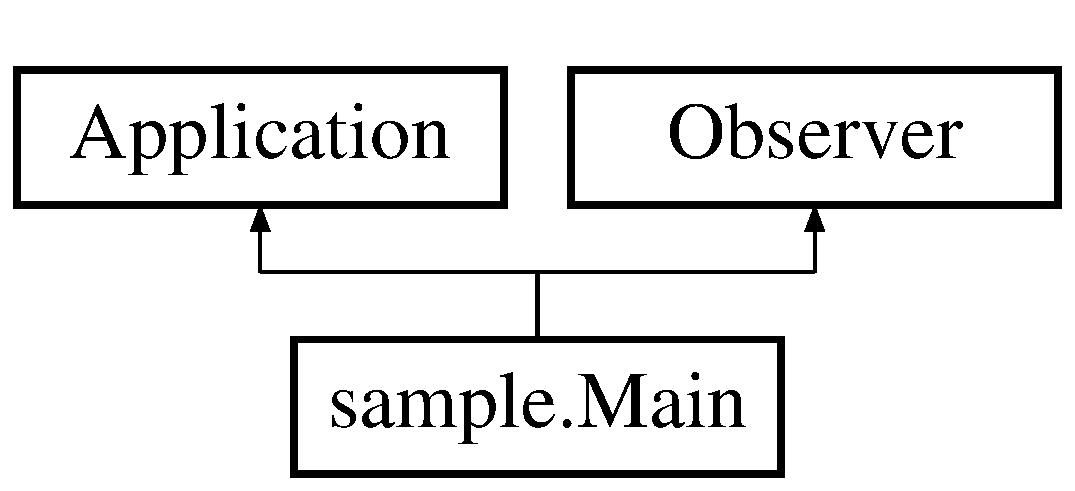
\includegraphics[height=2.000000cm]{classsample_1_1_main}
\end{center}
\end{figure}
\subsection*{Public Member Functions}
\begin{DoxyCompactItemize}
\item 
void \hyperlink{classsample_1_1_main_a4201e12604eb49ee4c0968db7aa3a876}{start} (Stage primary\+Stage)  throws Exception
\begin{DoxyCompactList}\small\item\em start the display \end{DoxyCompactList}\item 
void \hyperlink{classsample_1_1_main_a94132284ede73bbe43d239edc379351a}{update} (Observable o, Object arg)
\begin{DoxyCompactList}\small\item\em Start the game after login reception. \end{DoxyCompactList}\end{DoxyCompactItemize}
\subsection*{Static Public Member Functions}
\begin{DoxyCompactItemize}
\item 
static void \hyperlink{classsample_1_1_main_ab70e98057c0f40b833a38ea10a74eceb}{main} (String\mbox{[}$\,$\mbox{]} args)
\end{DoxyCompactItemize}


\subsection{Detailed Description}


Definition at line 23 of file Main.\+java.



\subsection{Member Function Documentation}
\index{sample\+::\+Main@{sample\+::\+Main}!main@{main}}
\index{main@{main}!sample\+::\+Main@{sample\+::\+Main}}
\subsubsection[{\texorpdfstring{main(\+String[] args)}{main(String[] args)}}]{\setlength{\rightskip}{0pt plus 5cm}static void sample.\+Main.\+main (
\begin{DoxyParamCaption}
\item[{String\mbox{[}$\,$\mbox{]}}]{args}
\end{DoxyParamCaption}
)\hspace{0.3cm}{\ttfamily [static]}}\hypertarget{classsample_1_1_main_ab70e98057c0f40b833a38ea10a74eceb}{}\label{classsample_1_1_main_ab70e98057c0f40b833a38ea10a74eceb}


Definition at line 52 of file Main.\+java.

\index{sample\+::\+Main@{sample\+::\+Main}!start@{start}}
\index{start@{start}!sample\+::\+Main@{sample\+::\+Main}}
\subsubsection[{\texorpdfstring{start(\+Stage primary\+Stage)}{start(Stage primaryStage)}}]{\setlength{\rightskip}{0pt plus 5cm}sample.\+Main.\+start (
\begin{DoxyParamCaption}
\item[{Stage}]{primary\+Stage}
\end{DoxyParamCaption}
) throws Exception}\hypertarget{classsample_1_1_main_a4201e12604eb49ee4c0968db7aa3a876}{}\label{classsample_1_1_main_a4201e12604eb49ee4c0968db7aa3a876}


start the display 


\begin{DoxyParams}{Parameters}
{\em primary\+Stage} & \\
\hline
\end{DoxyParams}

\begin{DoxyExceptions}{Exceptions}
{\em Exception} & \\
\hline
\end{DoxyExceptions}


Definition at line 37 of file Main.\+java.

\index{sample\+::\+Main@{sample\+::\+Main}!update@{update}}
\index{update@{update}!sample\+::\+Main@{sample\+::\+Main}}
\subsubsection[{\texorpdfstring{update(\+Observable o, Object arg)}{update(Observable o, Object arg)}}]{\setlength{\rightskip}{0pt plus 5cm}sample.\+Main.\+update (
\begin{DoxyParamCaption}
\item[{Observable}]{o, }
\item[{Object}]{arg}
\end{DoxyParamCaption}
)}\hypertarget{classsample_1_1_main_a94132284ede73bbe43d239edc379351a}{}\label{classsample_1_1_main_a94132284ede73bbe43d239edc379351a}


Start the game after login reception. 


\begin{DoxyParams}{Parameters}
{\em o} & \\
\hline
{\em arg} & \\
\hline
\end{DoxyParams}


Definition at line 64 of file Main.\+java.



The documentation for this class was generated from the following file\+:\begin{DoxyCompactItemize}
\item 
D\+:/owncloud/\+H\+E\+I\+G-\/\+V\+D/\+Java\+Projects/\+G\+E\+N\+\_\+\+Armagetron\+\_\+\+Client/src/main/java/sample/\hyperlink{_main_8java}{Main.\+java}\end{DoxyCompactItemize}

\hypertarget{classclient_1_1_player}{}\section{client.\+Player Class Reference}
\label{classclient_1_1_player}\index{client.\+Player@{client.\+Player}}
\subsection*{Public Member Functions}
\begin{DoxyCompactItemize}
\item 
\hyperlink{classclient_1_1_player_a13f87c3c7f92cf6efe4b73a2d4aca8a1}{Player} (U\+U\+ID unique\+Id, Point position, Color color, String username, boolean is\+Alive)
\item 
U\+U\+ID \hyperlink{classclient_1_1_player_a73afbf1a18acce12ba88c2b74fd41ce0}{get\+Unique\+Id} ()
\begin{DoxyCompactList}\small\item\em Get the Unique\+ID of the player. \end{DoxyCompactList}\item 
Color \hyperlink{classclient_1_1_player_a3c857d50ffcae64365e5a0914aa6f43e}{get\+Color} ()
\begin{DoxyCompactList}\small\item\em Return the color of the player. \end{DoxyCompactList}\item 
String \hyperlink{classclient_1_1_player_a0765c8775e3b2f52f6aa8c25b56d6375}{get\+Username} ()
\begin{DoxyCompactList}\small\item\em Return the player\textquotesingle{}s username. \end{DoxyCompactList}\item 
Point \hyperlink{classclient_1_1_player_a5eeedf6523a05e718de7386e234d8a8d}{get\+Position} ()
\begin{DoxyCompactList}\small\item\em Return the player\textquotesingle{}s position. \end{DoxyCompactList}\item 
boolean \hyperlink{classclient_1_1_player_a21e80dfdf04a4a9d3eff3dad411f7232}{is\+Alive} ()
\end{DoxyCompactItemize}


\subsection{Detailed Description}


Definition at line 14 of file Player.\+java.



\subsection{Constructor \& Destructor Documentation}
\index{client\+::\+Player@{client\+::\+Player}!Player@{Player}}
\index{Player@{Player}!client\+::\+Player@{client\+::\+Player}}
\subsubsection[{\texorpdfstring{Player(\+U\+U\+I\+D unique\+Id, Point position, Color color, String username, boolean is\+Alive)}{Player(UUID uniqueId, Point position, Color color, String username, boolean isAlive)}}]{\setlength{\rightskip}{0pt plus 5cm}client.\+Player.\+Player (
\begin{DoxyParamCaption}
\item[{U\+U\+ID}]{unique\+Id, }
\item[{Point}]{position, }
\item[{Color}]{color, }
\item[{String}]{username, }
\item[{boolean}]{is\+Alive}
\end{DoxyParamCaption}
)}\hypertarget{classclient_1_1_player_a13f87c3c7f92cf6efe4b73a2d4aca8a1}{}\label{classclient_1_1_player_a13f87c3c7f92cf6efe4b73a2d4aca8a1}


Definition at line 21 of file Player.\+java.



\subsection{Member Function Documentation}
\index{client\+::\+Player@{client\+::\+Player}!get\+Color@{get\+Color}}
\index{get\+Color@{get\+Color}!client\+::\+Player@{client\+::\+Player}}
\subsubsection[{\texorpdfstring{get\+Color()}{getColor()}}]{\setlength{\rightskip}{0pt plus 5cm}client.\+Player.\+get\+Color (
\begin{DoxyParamCaption}
{}
\end{DoxyParamCaption}
)}\hypertarget{classclient_1_1_player_a3c857d50ffcae64365e5a0914aa6f43e}{}\label{classclient_1_1_player_a3c857d50ffcae64365e5a0914aa6f43e}


Return the color of the player. 

\begin{DoxyReturn}{Returns}
Color 
\end{DoxyReturn}


Definition at line 47 of file Player.\+java.

\index{client\+::\+Player@{client\+::\+Player}!get\+Position@{get\+Position}}
\index{get\+Position@{get\+Position}!client\+::\+Player@{client\+::\+Player}}
\subsubsection[{\texorpdfstring{get\+Position()}{getPosition()}}]{\setlength{\rightskip}{0pt plus 5cm}client.\+Player.\+get\+Position (
\begin{DoxyParamCaption}
{}
\end{DoxyParamCaption}
)}\hypertarget{classclient_1_1_player_a5eeedf6523a05e718de7386e234d8a8d}{}\label{classclient_1_1_player_a5eeedf6523a05e718de7386e234d8a8d}


Return the player\textquotesingle{}s position. 

\begin{DoxyReturn}{Returns}
Point 
\end{DoxyReturn}


Definition at line 69 of file Player.\+java.

\index{client\+::\+Player@{client\+::\+Player}!get\+Unique\+Id@{get\+Unique\+Id}}
\index{get\+Unique\+Id@{get\+Unique\+Id}!client\+::\+Player@{client\+::\+Player}}
\subsubsection[{\texorpdfstring{get\+Unique\+Id()}{getUniqueId()}}]{\setlength{\rightskip}{0pt plus 5cm}client.\+Player.\+get\+Unique\+Id (
\begin{DoxyParamCaption}
{}
\end{DoxyParamCaption}
)}\hypertarget{classclient_1_1_player_a73afbf1a18acce12ba88c2b74fd41ce0}{}\label{classclient_1_1_player_a73afbf1a18acce12ba88c2b74fd41ce0}


Get the Unique\+ID of the player. 

\begin{DoxyReturn}{Returns}
U\+U\+ID 
\end{DoxyReturn}


Definition at line 36 of file Player.\+java.

\index{client\+::\+Player@{client\+::\+Player}!get\+Username@{get\+Username}}
\index{get\+Username@{get\+Username}!client\+::\+Player@{client\+::\+Player}}
\subsubsection[{\texorpdfstring{get\+Username()}{getUsername()}}]{\setlength{\rightskip}{0pt plus 5cm}client.\+Player.\+get\+Username (
\begin{DoxyParamCaption}
{}
\end{DoxyParamCaption}
)}\hypertarget{classclient_1_1_player_a0765c8775e3b2f52f6aa8c25b56d6375}{}\label{classclient_1_1_player_a0765c8775e3b2f52f6aa8c25b56d6375}


Return the player\textquotesingle{}s username. 

\begin{DoxyReturn}{Returns}
String 
\end{DoxyReturn}


Definition at line 58 of file Player.\+java.

\index{client\+::\+Player@{client\+::\+Player}!is\+Alive@{is\+Alive}}
\index{is\+Alive@{is\+Alive}!client\+::\+Player@{client\+::\+Player}}
\subsubsection[{\texorpdfstring{is\+Alive()}{isAlive()}}]{\setlength{\rightskip}{0pt plus 5cm}boolean client.\+Player.\+is\+Alive (
\begin{DoxyParamCaption}
{}
\end{DoxyParamCaption}
)}\hypertarget{classclient_1_1_player_a21e80dfdf04a4a9d3eff3dad411f7232}{}\label{classclient_1_1_player_a21e80dfdf04a4a9d3eff3dad411f7232}


Definition at line 80 of file Player.\+java.



The documentation for this class was generated from the following file\+:\begin{DoxyCompactItemize}
\item 
D\+:/owncloud/\+H\+E\+I\+G-\/\+V\+D/\+Java\+Projects/\+G\+E\+N\+\_\+\+Armagetron\+\_\+\+Client/src/main/java/client/\hyperlink{_player_8java}{Player.\+java}\end{DoxyCompactItemize}

\hypertarget{classclient_1_1_player_test}{}\section{client.\+Player\+Test Class Reference}
\label{classclient_1_1_player_test}\index{client.\+Player\+Test@{client.\+Player\+Test}}
\subsection*{Public Member Functions}
\begin{DoxyCompactItemize}
\item 
void \hyperlink{classclient_1_1_player_test_af4ead338a74eb5e64c96e4da202fb3c9}{get\+Unique\+Id} ()  throws Exception 
\item 
void \hyperlink{classclient_1_1_player_test_ab60031303a506646bdeb34ce47bfaa26}{get\+Color} ()  throws Exception 
\item 
void \hyperlink{classclient_1_1_player_test_a4fa505e723da85fcd90954ae6b158e1b}{get\+Username} ()  throws Exception 
\item 
void \hyperlink{classclient_1_1_player_test_aace6db46e241ef50a4bb7292f4e075f1}{get\+Position} ()  throws Exception 
\item 
void \hyperlink{classclient_1_1_player_test_a8df6b5fa004a179f5dd51efcaeb9eae3}{is\+Alive} ()  throws Exception 
\end{DoxyCompactItemize}


\subsection{Detailed Description}


Definition at line 20 of file Player\+Test.\+java.



\subsection{Member Function Documentation}
\index{client\+::\+Player\+Test@{client\+::\+Player\+Test}!get\+Color@{get\+Color}}
\index{get\+Color@{get\+Color}!client\+::\+Player\+Test@{client\+::\+Player\+Test}}
\subsubsection[{\texorpdfstring{get\+Color()}{getColor()}}]{\setlength{\rightskip}{0pt plus 5cm}void client.\+Player\+Test.\+get\+Color (
\begin{DoxyParamCaption}
{}
\end{DoxyParamCaption}
) throws Exception}\hypertarget{classclient_1_1_player_test_ab60031303a506646bdeb34ce47bfaa26}{}\label{classclient_1_1_player_test_ab60031303a506646bdeb34ce47bfaa26}


Definition at line 32 of file Player\+Test.\+java.

\index{client\+::\+Player\+Test@{client\+::\+Player\+Test}!get\+Position@{get\+Position}}
\index{get\+Position@{get\+Position}!client\+::\+Player\+Test@{client\+::\+Player\+Test}}
\subsubsection[{\texorpdfstring{get\+Position()}{getPosition()}}]{\setlength{\rightskip}{0pt plus 5cm}void client.\+Player\+Test.\+get\+Position (
\begin{DoxyParamCaption}
{}
\end{DoxyParamCaption}
) throws Exception}\hypertarget{classclient_1_1_player_test_aace6db46e241ef50a4bb7292f4e075f1}{}\label{classclient_1_1_player_test_aace6db46e241ef50a4bb7292f4e075f1}


Definition at line 42 of file Player\+Test.\+java.

\index{client\+::\+Player\+Test@{client\+::\+Player\+Test}!get\+Unique\+Id@{get\+Unique\+Id}}
\index{get\+Unique\+Id@{get\+Unique\+Id}!client\+::\+Player\+Test@{client\+::\+Player\+Test}}
\subsubsection[{\texorpdfstring{get\+Unique\+Id()}{getUniqueId()}}]{\setlength{\rightskip}{0pt plus 5cm}void client.\+Player\+Test.\+get\+Unique\+Id (
\begin{DoxyParamCaption}
{}
\end{DoxyParamCaption}
) throws Exception}\hypertarget{classclient_1_1_player_test_af4ead338a74eb5e64c96e4da202fb3c9}{}\label{classclient_1_1_player_test_af4ead338a74eb5e64c96e4da202fb3c9}


Definition at line 27 of file Player\+Test.\+java.

\index{client\+::\+Player\+Test@{client\+::\+Player\+Test}!get\+Username@{get\+Username}}
\index{get\+Username@{get\+Username}!client\+::\+Player\+Test@{client\+::\+Player\+Test}}
\subsubsection[{\texorpdfstring{get\+Username()}{getUsername()}}]{\setlength{\rightskip}{0pt plus 5cm}void client.\+Player\+Test.\+get\+Username (
\begin{DoxyParamCaption}
{}
\end{DoxyParamCaption}
) throws Exception}\hypertarget{classclient_1_1_player_test_a4fa505e723da85fcd90954ae6b158e1b}{}\label{classclient_1_1_player_test_a4fa505e723da85fcd90954ae6b158e1b}


Definition at line 37 of file Player\+Test.\+java.

\index{client\+::\+Player\+Test@{client\+::\+Player\+Test}!is\+Alive@{is\+Alive}}
\index{is\+Alive@{is\+Alive}!client\+::\+Player\+Test@{client\+::\+Player\+Test}}
\subsubsection[{\texorpdfstring{is\+Alive()}{isAlive()}}]{\setlength{\rightskip}{0pt plus 5cm}void client.\+Player\+Test.\+is\+Alive (
\begin{DoxyParamCaption}
{}
\end{DoxyParamCaption}
) throws Exception}\hypertarget{classclient_1_1_player_test_a8df6b5fa004a179f5dd51efcaeb9eae3}{}\label{classclient_1_1_player_test_a8df6b5fa004a179f5dd51efcaeb9eae3}


Definition at line 47 of file Player\+Test.\+java.



The documentation for this class was generated from the following file\+:\begin{DoxyCompactItemize}
\item 
D\+:/owncloud/\+H\+E\+I\+G-\/\+V\+D/\+Java\+Projects/\+G\+E\+N\+\_\+\+Armagetron\+\_\+\+Client/src/test/java/client/\hyperlink{_player_test_8java}{Player\+Test.\+java}\end{DoxyCompactItemize}

\chapter{File Documentation}
\hypertarget{_r_e_a_d_m_e_8md}{}\section{D\+:/owncloud/\+H\+E\+I\+G-\/\+V\+D/\+Java\+Projects/\+G\+E\+N\+\_\+\+Armagetron\+\_\+\+Client/\+R\+E\+A\+D\+ME.md File Reference}
\label{_r_e_a_d_m_e_8md}\index{D\+:/owncloud/\+H\+E\+I\+G-\/\+V\+D/\+Java\+Projects/\+G\+E\+N\+\_\+\+Armagetron\+\_\+\+Client/\+R\+E\+A\+D\+M\+E.\+md@{D\+:/owncloud/\+H\+E\+I\+G-\/\+V\+D/\+Java\+Projects/\+G\+E\+N\+\_\+\+Armagetron\+\_\+\+Client/\+R\+E\+A\+D\+M\+E.\+md}}

\hypertarget{_client_8java}{}\section{D\+:/owncloud/\+H\+E\+I\+G-\/\+V\+D/\+Java\+Projects/\+G\+E\+N\+\_\+\+Armagetron\+\_\+\+Client/src/main/java/client/\+Client.java File Reference}
\label{_client_8java}\index{D\+:/owncloud/\+H\+E\+I\+G-\/\+V\+D/\+Java\+Projects/\+G\+E\+N\+\_\+\+Armagetron\+\_\+\+Client/src/main/java/client/\+Client.\+java@{D\+:/owncloud/\+H\+E\+I\+G-\/\+V\+D/\+Java\+Projects/\+G\+E\+N\+\_\+\+Armagetron\+\_\+\+Client/src/main/java/client/\+Client.\+java}}


\+: Client Class that generate the play ground window  


\subsection*{Classes}
\begin{DoxyCompactItemize}
\item 
class \hyperlink{classclient_1_1_client}{client.\+Client}
\end{DoxyCompactItemize}
\subsection*{Packages}
\begin{DoxyCompactItemize}
\item 
package \hyperlink{namespaceclient}{client}
\end{DoxyCompactItemize}


\subsection{Detailed Description}
\+: Client Class that generate the play ground window 

\+: Argmagetron

\begin{DoxyAuthor}{Author}
(s) \+: Thomas Lechaire, Kevin Pradervand, Elie N\textquotesingle{}Djoli Bohulu, Michael Brouchoud 
\end{DoxyAuthor}
\begin{DoxyDate}{Date}
\+: 08.\+06.\+2017 
\end{DoxyDate}

\hypertarget{_game_8java}{}\section{D\+:/owncloud/\+H\+E\+I\+G-\/\+V\+D/\+Java\+Projects/\+G\+E\+N\+\_\+\+Armagetron\+\_\+\+Client/src/main/java/client/\+Game.java File Reference}
\label{_game_8java}\index{D\+:/owncloud/\+H\+E\+I\+G-\/\+V\+D/\+Java\+Projects/\+G\+E\+N\+\_\+\+Armagetron\+\_\+\+Client/src/main/java/client/\+Game.\+java@{D\+:/owncloud/\+H\+E\+I\+G-\/\+V\+D/\+Java\+Projects/\+G\+E\+N\+\_\+\+Armagetron\+\_\+\+Client/src/main/java/client/\+Game.\+java}}


\+: Game class that manage local data for players  


\subsection*{Classes}
\begin{DoxyCompactItemize}
\item 
class \hyperlink{classclient_1_1_game}{client.\+Game}
\end{DoxyCompactItemize}
\subsection*{Packages}
\begin{DoxyCompactItemize}
\item 
package \hyperlink{namespaceclient}{client}
\end{DoxyCompactItemize}


\subsection{Detailed Description}
\+: Game class that manage local data for players 

\+: The class Game

\+: Argmagetron

\begin{DoxyAuthor}{Author}
(s) \+: Thomas Lechaire, Kevin Pradervand, Elie N\textquotesingle{}Djoli Bohulu, Michael Brouchoud 
\end{DoxyAuthor}
\begin{DoxyDate}{Date}
\+: 08.\+06.\+2017
\end{DoxyDate}
\+: Argmagetron

\begin{DoxyAuthor}{Author}
(s) \+: Kevin Pradervand 
\end{DoxyAuthor}
\begin{DoxyDate}{Date}
\+: 18.\+05.\+2017 
\end{DoxyDate}

\hypertarget{_player_8java}{}\section{D\+:/owncloud/\+H\+E\+I\+G-\/\+V\+D/\+Java\+Projects/\+G\+E\+N\+\_\+\+Armagetron\+\_\+\+Client/src/main/java/client/\+Player.java File Reference}
\label{_player_8java}\index{D\+:/owncloud/\+H\+E\+I\+G-\/\+V\+D/\+Java\+Projects/\+G\+E\+N\+\_\+\+Armagetron\+\_\+\+Client/src/main/java/client/\+Player.\+java@{D\+:/owncloud/\+H\+E\+I\+G-\/\+V\+D/\+Java\+Projects/\+G\+E\+N\+\_\+\+Armagetron\+\_\+\+Client/src/main/java/client/\+Player.\+java}}


\+: Player class  


\subsection*{Classes}
\begin{DoxyCompactItemize}
\item 
class \hyperlink{classclient_1_1_player}{client.\+Player}
\end{DoxyCompactItemize}
\subsection*{Packages}
\begin{DoxyCompactItemize}
\item 
package \hyperlink{namespaceclient}{client}
\end{DoxyCompactItemize}


\subsection{Detailed Description}
\+: Player class 

\+: The class Player

\+: Argmagetron

\begin{DoxyAuthor}{Author}
(s) \+: Thomas Lechaire, Kevin Pradervand, Elie N\textquotesingle{}Djoli Bohulu, Michael Brouchoud 
\end{DoxyAuthor}
\begin{DoxyDate}{Date}
\+: 08.\+06.\+2017
\end{DoxyDate}
\+: Argmagetron

\begin{DoxyAuthor}{Author}
(s) \+: Kevin Pradervand 
\end{DoxyAuthor}
\begin{DoxyDate}{Date}
\+: 18.\+05.\+2017 
\end{DoxyDate}

\hypertarget{_login_controller_8java}{}\section{D\+:/owncloud/\+H\+E\+I\+G-\/\+V\+D/\+Java\+Projects/\+G\+E\+N\+\_\+\+Armagetron\+\_\+\+Client/src/main/java/login/\+Login\+Controller.java File Reference}
\label{_login_controller_8java}\index{D\+:/owncloud/\+H\+E\+I\+G-\/\+V\+D/\+Java\+Projects/\+G\+E\+N\+\_\+\+Armagetron\+\_\+\+Client/src/main/java/login/\+Login\+Controller.\+java@{D\+:/owncloud/\+H\+E\+I\+G-\/\+V\+D/\+Java\+Projects/\+G\+E\+N\+\_\+\+Armagetron\+\_\+\+Client/src/main/java/login/\+Login\+Controller.\+java}}


\+: Controller of the login windows  


\subsection*{Classes}
\begin{DoxyCompactItemize}
\item 
class \hyperlink{classlogin_1_1_login_controller}{login.\+Login\+Controller}
\end{DoxyCompactItemize}
\subsection*{Packages}
\begin{DoxyCompactItemize}
\item 
package \hyperlink{namespacelogin}{login}
\end{DoxyCompactItemize}


\subsection{Detailed Description}
\+: Controller of the login windows 

\+: The class Login\+Controller

\+: Argmagetron

\begin{DoxyAuthor}{Author}
(s) \+: Thomas Lechaire, Kevin Pradervand, Elie N\textquotesingle{}Djoli Bohulu, Michael Brouchoud 
\end{DoxyAuthor}
\begin{DoxyDate}{Date}
\+: 08.\+06.\+2017
\end{DoxyDate}
\+: Argmagetron

\begin{DoxyAuthor}{Author}
(s) \+: Kevin Pradervand 
\end{DoxyAuthor}
\begin{DoxyDate}{Date}
\+: 18.\+05.\+2017 
\end{DoxyDate}

\hypertarget{_controller_8java}{}\section{D\+:/owncloud/\+H\+E\+I\+G-\/\+V\+D/\+Java\+Projects/\+G\+E\+N\+\_\+\+Armagetron\+\_\+\+Client/src/main/java/sample/\+Controller.java File Reference}
\label{_controller_8java}\index{D\+:/owncloud/\+H\+E\+I\+G-\/\+V\+D/\+Java\+Projects/\+G\+E\+N\+\_\+\+Armagetron\+\_\+\+Client/src/main/java/sample/\+Controller.\+java@{D\+:/owncloud/\+H\+E\+I\+G-\/\+V\+D/\+Java\+Projects/\+G\+E\+N\+\_\+\+Armagetron\+\_\+\+Client/src/main/java/sample/\+Controller.\+java}}


\+: Controller of the playing grid that display the game  


\subsection*{Classes}
\begin{DoxyCompactItemize}
\item 
class \hyperlink{classsample_1_1_controller}{sample.\+Controller}
\end{DoxyCompactItemize}
\subsection*{Packages}
\begin{DoxyCompactItemize}
\item 
package \hyperlink{namespacesample}{sample}
\end{DoxyCompactItemize}


\subsection{Detailed Description}
\+: Controller of the playing grid that display the game 

\+: The class Controller

\+: Argmagetron

\begin{DoxyAuthor}{Author}
(s) \+: Thomas Lechaire, Kevin Pradervand, Elie N\textquotesingle{}Djoli Bohulu, Michael Brouchoud 
\end{DoxyAuthor}
\begin{DoxyDate}{Date}
\+: 08.\+06.\+2017
\end{DoxyDate}
\+: Argmagetron

\begin{DoxyAuthor}{Author}
(s) \+: Kevin Pradervand 
\end{DoxyAuthor}
\begin{DoxyDate}{Date}
\+: 18.\+05.\+2017 
\end{DoxyDate}

\hypertarget{_main_8java}{}\section{D\+:/owncloud/\+H\+E\+I\+G-\/\+V\+D/\+Java\+Projects/\+G\+E\+N\+\_\+\+Armagetron\+\_\+\+Client/src/main/java/sample/\+Main.java File Reference}
\label{_main_8java}\index{D\+:/owncloud/\+H\+E\+I\+G-\/\+V\+D/\+Java\+Projects/\+G\+E\+N\+\_\+\+Armagetron\+\_\+\+Client/src/main/java/sample/\+Main.\+java@{D\+:/owncloud/\+H\+E\+I\+G-\/\+V\+D/\+Java\+Projects/\+G\+E\+N\+\_\+\+Armagetron\+\_\+\+Client/src/main/java/sample/\+Main.\+java}}


\+: M\+A\+IN class that run the client  


\subsection*{Classes}
\begin{DoxyCompactItemize}
\item 
class \hyperlink{classsample_1_1_main}{sample.\+Main}
\end{DoxyCompactItemize}
\subsection*{Packages}
\begin{DoxyCompactItemize}
\item 
package \hyperlink{namespacesample}{sample}
\end{DoxyCompactItemize}


\subsection{Detailed Description}
\+: M\+A\+IN class that run the client 

\+: Argmagetron

\begin{DoxyAuthor}{Author}
(s) \+: Thomas Lechaire, Kevin Pradervand, Elie N\textquotesingle{}Djoli Bohulu, Michael Brouchoud 
\end{DoxyAuthor}
\begin{DoxyDate}{Date}
\+: 08.\+06.\+2017 
\end{DoxyDate}

\hypertarget{_game_test_8java}{}\section{D\+:/owncloud/\+H\+E\+I\+G-\/\+V\+D/\+Java\+Projects/\+G\+E\+N\+\_\+\+Armagetron\+\_\+\+Client/src/test/java/client/\+Game\+Test.java File Reference}
\label{_game_test_8java}\index{D\+:/owncloud/\+H\+E\+I\+G-\/\+V\+D/\+Java\+Projects/\+G\+E\+N\+\_\+\+Armagetron\+\_\+\+Client/src/test/java/client/\+Game\+Test.\+java@{D\+:/owncloud/\+H\+E\+I\+G-\/\+V\+D/\+Java\+Projects/\+G\+E\+N\+\_\+\+Armagetron\+\_\+\+Client/src/test/java/client/\+Game\+Test.\+java}}
\subsection*{Classes}
\begin{DoxyCompactItemize}
\item 
class \hyperlink{classclient_1_1_game_test}{client.\+Game\+Test}
\end{DoxyCompactItemize}
\subsection*{Packages}
\begin{DoxyCompactItemize}
\item 
package \hyperlink{namespaceclient}{client}
\end{DoxyCompactItemize}

\hypertarget{_player_test_8java}{}\section{D\+:/owncloud/\+H\+E\+I\+G-\/\+V\+D/\+Java\+Projects/\+G\+E\+N\+\_\+\+Armagetron\+\_\+\+Client/src/test/java/client/\+Player\+Test.java File Reference}
\label{_player_test_8java}\index{D\+:/owncloud/\+H\+E\+I\+G-\/\+V\+D/\+Java\+Projects/\+G\+E\+N\+\_\+\+Armagetron\+\_\+\+Client/src/test/java/client/\+Player\+Test.\+java@{D\+:/owncloud/\+H\+E\+I\+G-\/\+V\+D/\+Java\+Projects/\+G\+E\+N\+\_\+\+Armagetron\+\_\+\+Client/src/test/java/client/\+Player\+Test.\+java}}
\subsection*{Classes}
\begin{DoxyCompactItemize}
\item 
class \hyperlink{classclient_1_1_player_test}{client.\+Player\+Test}
\end{DoxyCompactItemize}
\subsection*{Packages}
\begin{DoxyCompactItemize}
\item 
package \hyperlink{namespaceclient}{client}
\end{DoxyCompactItemize}

\hypertarget{_login_controller_test_8java}{}\section{D\+:/owncloud/\+H\+E\+I\+G-\/\+V\+D/\+Java\+Projects/\+G\+E\+N\+\_\+\+Armagetron\+\_\+\+Client/src/test/java/login/\+Login\+Controller\+Test.java File Reference}
\label{_login_controller_test_8java}\index{D\+:/owncloud/\+H\+E\+I\+G-\/\+V\+D/\+Java\+Projects/\+G\+E\+N\+\_\+\+Armagetron\+\_\+\+Client/src/test/java/login/\+Login\+Controller\+Test.\+java@{D\+:/owncloud/\+H\+E\+I\+G-\/\+V\+D/\+Java\+Projects/\+G\+E\+N\+\_\+\+Armagetron\+\_\+\+Client/src/test/java/login/\+Login\+Controller\+Test.\+java}}
\subsection*{Classes}
\begin{DoxyCompactItemize}
\item 
class \hyperlink{classlogin_1_1_login_controller_test}{login.\+Login\+Controller\+Test}
\end{DoxyCompactItemize}
\subsection*{Packages}
\begin{DoxyCompactItemize}
\item 
package \hyperlink{namespacelogin}{login}
\end{DoxyCompactItemize}

\hypertarget{_controller_test_8java}{}\section{D\+:/owncloud/\+H\+E\+I\+G-\/\+V\+D/\+Java\+Projects/\+G\+E\+N\+\_\+\+Armagetron\+\_\+\+Client/src/test/java/sample/\+Controller\+Test.java File Reference}
\label{_controller_test_8java}\index{D\+:/owncloud/\+H\+E\+I\+G-\/\+V\+D/\+Java\+Projects/\+G\+E\+N\+\_\+\+Armagetron\+\_\+\+Client/src/test/java/sample/\+Controller\+Test.\+java@{D\+:/owncloud/\+H\+E\+I\+G-\/\+V\+D/\+Java\+Projects/\+G\+E\+N\+\_\+\+Armagetron\+\_\+\+Client/src/test/java/sample/\+Controller\+Test.\+java}}
\subsection*{Classes}
\begin{DoxyCompactItemize}
\item 
class \hyperlink{classsample_1_1_controller_test}{sample.\+Controller\+Test}
\end{DoxyCompactItemize}
\subsection*{Packages}
\begin{DoxyCompactItemize}
\item 
package \hyperlink{namespacesample}{sample}
\end{DoxyCompactItemize}

%--- End generated contents ---

% Index
\backmatter
\newpage
\phantomsection
\clearemptydoublepage
\addcontentsline{toc}{chapter}{Index}
\printindex

\end{document}
